\documentclass[koma,a4paper]{article}
\usepackage[T1]{fontenc}
\usepackage{fixltx2e}
\usepackage{graphicx}
\usepackage{float}
\usepackage{amsmath}
\usepackage{amssymb}
\usepackage[hidelinks]{hyperref}
\usepackage{amsthm}
\usepackage{tikz}
\usepackage{todonotes}
\usepackage{booktabs}
\usepackage{subcaption}
\usepackage{color}
\usepackage{lmodern}
\usepackage{mathtools}
\graphicspath{{graphics/}}
\usetikzlibrary{trees}

\newcommand*\circled[1]{\tikz[baseline=(char.base)]{\node[shape=circle,draw,inner sep=2pt] (char) {#1};}} % circles around numbers

\title{AALG Self Study 3}
\author{Andreas Petersen\\
Mads E. Kalør\\
Søren B. Ranneries\\
Room 1.1.34}
\begin{document}
\maketitle

\pagebreak

\section{Exercise 1}
The answer is c.

\section{Exercise 2}

\subsection{a}
Figure \ref{fig:vertices_capacity} shows how to convert a vertex with capacity to a regular flow network. The number of edges in a network with vertex capacities is $2|V|$ in a regular flow network, and the number of edges is $|V|+|E|$.

\begin{figure}
  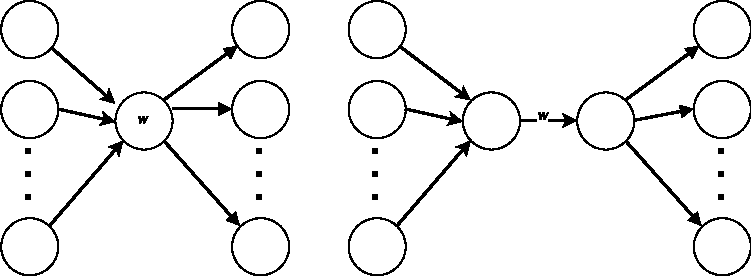
\includegraphics{weighted_vertices}
  \caption{Vertices with capacity}
  \label{fig:vertices_capacity}
\end{figure}

\subsection{b}
We make an algorithm that reduces the \emph{escape problem}  to the \emph{flow} problem, and then run an Edmond-Karp algorithm on the resulting graph. All edges have implicitly the capacity 1.

We have to give the vertices a capacity of 1 (as seen in exercise 2.a) and convert the undirected edges to two directed edges as seen in Figure \ref{fig:two_way1}. However, we have found that this is automatically handled when we convert a vertex into an input-vertex and an output vertex (to handle vertex capacity), as seen in Figure \ref{fig:two_way1}.
\begin{figure}
  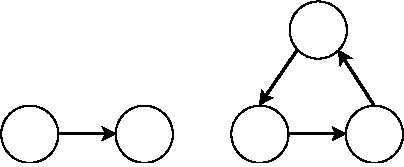
\includegraphics{two_way_path}
  \caption{Conversion of undirected graph to directed graph}
  \label{fig:two_way1}
\end{figure}
\begin{figure}
  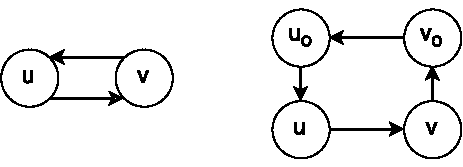
\includegraphics{two_way_path2}
  \caption{How direction is automatically handled}
  \label{fig:two_way2}
\end{figure}

\begin{enumerate}
  \item Create a new graph $G' = (V', E')$. $V'$ and $E'$ are initially empty.
  \item For each $v \in V$ add vertices $v$ and $v_o$ to $V'$ and edge $(v, v_o)$ to $E'$
  \item For each $v \in V$
  \begin{enumerate}
    \item For each $(v, u) \in E$ add $(v_o, u)$ to $E'$
  \end{enumerate}
  \item Add a source vertex, $s$, to $V'$ and for each vertex $p \in \mathit{startingPoints} \subseteq V$ add an edge $(s, p)$ to $E'$
  \item Add a sink vertex, $t$, to $V'$ and for each vertex $b \in \mathit{boundaryVertices} \subseteq V$ add an edge $(b, t)$ to $E'$
  \item Run $G'$ on the Edmond-Karp algorithm and if the answer equals the number of starting points, then return true. Otherwise false.
\end{enumerate}

The complexity of the algorithm is a simply analysis of each point:

\begin{enumerate}
  \item $\Theta(1)$
  \item $\Theta\left(|V|\right)$
  \item $\Theta\left(|V| + |E|\right)$
  \item $O(|V|)$
  \item $\Theta\left(\sqrt{|V|}\right)$
  \item $O\left(|V||E|\right)$. The maximum flow is equal to $|V|$ and since the worst-case running time of the Ford-Fulkerson method is $O\left(|E||f*|\right)$.
\end{enumerate}

Thus the complete running time of the algorithm is $O\left(|V||E|\right)$.

\section{Exercise 3}
\subsection{a}
\begin{align*}
  &\text{SearchDynamic}(s)\\
  &~~~~\text{for } i \leftarrow 0 \text{ to } k\\
  &~~~~~~~~\text{if } n_i = 1 \text{ then}\\
  &~~~~~~~~~~~~x \leftarrow \text{search}(A_i, s)\\
  &~~~~~~~~~~~~\text{if } x \neq \text{null} \text{ then}\\
  &~~~~~~~~~~~~~~~~\text{return } x\\
  &~~~~\text{return null}
\end{align*}

The worst case running time of SearchDynamic is: $$\log{2}^0 + \log{2}^1 + \dots + \log{k} = 0 + 1 + \dots + k = \Theta\left(k\right) = \Theta\left(\left\lceil\log{(n+1)}^2\right\rceil\right)$$

\subsection{b}
The $\text{merge}(A_1, A_2)$ procedure merges array $A_1$ into array $A_2$ and is similar to the merge procedure in the mergesort algorithm. It runs in $\Theta(n)$ time, where $n$ is $A_1.\text{length} + A_2.\text{length}$ (where the length is the number of elements in each array, and not necessarily equal to the allocated size of the array).
\begin{align*}
  &\text{Insert}(x)\\
  &~~~~i \leftarrow 0\\
  &~~~~\text{while } n_i = 1 \text{ and } i < k\\
  &~~~~~~~~i \leftarrow i + 1\\
  &~~~~\text{if } i = k \text{ then}\\
  &~~~~~~~~A_k \leftarrow \text{ new array of size } 2^k\\
  &~~~~~~~~k \leftarrow k + 1\\
  &~~~~n_i \leftarrow 1\\
  &~~~~A_i[0] \leftarrow x\\
  &~~~~\text{for } j \leftarrow i - 1 \text{ to } 0\\
  &~~~~~~~~\text{merge}(A_j, A_i)\\
  &~~~~~~~~n_j \leftarrow 0\\
\end{align*}

Worst case running time: In worst case, we merge $k$ times. First time we merge arrays of length $2^{k-1}$ and $1$. Second time arrays of length $2^{k-2}$ and $2^{k-1}+1$, then $2^{k-3}$ and $2^{k-2}+2^{k-1}+1$, and so on. This gives the sum:
\begin{align*}
&\sum_{i=1}^{k}(1+2^k-2^{i-1})\\
&= 2^kk+k - \sum_{i=1}^{k} 2^{i-1}\\
&=2^kk+k-\frac{2^k-1}{2-1}\\
&=2^kk+k-2^k+1\\
&=2^k(k-1)+k+1\\
&=2^{\log(n+1)}(\log(n+1)-1)+\log(n+1)+1\\
&=(n+1)(\log(n+1)-1)+\log(n+1)+1\\
&=\Theta\left(n\log n\right)
\end{align*}
\\\\
Amortized running time: For convenience, we assume that insertion into an empty array is a merge of 1 element. We assume $n$ operations starting from $k=1, n_k=0$. Every second time, we merge one element to an empty array. Every fourth time, we merge $1+2$ elements (first one element to the empty array, then $A_1$ with the new array), and every eighth time, we merge $1+2+4$ elements and so on: $\frac{n}{2}1+\frac{n}{4}(1+2)+\frac{n}{8}(1+2+4) \ldots$. This is equal to:
\begin{align*}
  &n \sum_{i=1}^{\log(n+1)} \frac{\sum_{j=0}^{i-1}2^j}{2^i}\\
  &=n \sum_{i=1}^{\log(n+1)} \frac{\frac{2^i-1}{2-1}}{2^i}\\
\end{align*}
When constants are removed, we have the following number of operations in the sequence:
\begin{align*}
  &\Theta\left(n \sum_{i=1}^{\log(n+1)} \frac{2^i}{2^i}\right)\\
  &=\Theta\left(n \log n\right)
\end{align*}
We divide this with $n$ operations and the amortized cost per operation is $\Theta\left(\log n\right)$.

\subsection{c}
% BinarySearch(x, A) returns element index or -1
Idea: First find element $y$ in array $A_i$ on index $p$. Then remove the element from $A_i$ and move all elements before $y$ up, and then put $y$ at index 0. Then we call the auxillary function which takes a list of arrays $A_0$ to $A_m$ and removes the first element of $A_m$ and propagates the other elements into the arrays $A_0$ to $A_{m-1}$.
\begin{align*}
  &\text{Delete}(x)\\
  &~~~~\text{for } i=0 \text{ to } k-1\\
  &~~~~~~~~p \leftarrow \text{BinarySearch}(x, A_i)\\
  &~~~~~~~~\text{if } p \neq -1 \text{ then}\\
  &~~~~~~~~~~~~y \leftarrow A_i[p]\\
  &~~~~~~~~~~~~\text{for } q=p-1 \text{ to } 0\\
  &~~~~~~~~~~~~~~~~A_i[q+1] \leftarrow A_i[q]\\
  &~~~~~~~~~~~~A_i[0] \leftarrow y\\
  &~~~~~~~~~~~~\text{break}\\
  &~~~~\text{DeleteAux}(A_0\ldots A_i)\\
\end{align*}
The insert($x, A$) function inserts element $x$ into an already sorted array $A$ with one free element in worst case $O(n)$ time.
\begin{align*}
  &\text{DeleteAux}(A_0\ldots A_m)\\
  &~~~~i \leftarrow m-1\\
  &~~~~\text{while } n_i = 0 \text{ and } i > 0\\
  &~~~~~~~~i \leftarrow i - 1\\
  &~~~~y \leftarrow A_i[0]\\
  &~~~~\text{if } i = 0 \text{ then}\\
  &~~~~~~~~p \leftarrow 1\\
  &~~~~~~~~\text{for } j=m-1 \text{ to } 0\\
  &~~~~~~~~~~~~A_j \leftarrow A_m[p:2^j]\\
  &~~~~~~~~~~~~n_j \leftarrow 1\\
  &~~~~~~~~~~~~p \leftarrow 2^j\\
  &~~~~~~~~n_0 \leftarrow 0\\
  &~~~~\text{else then}\\
  &~~~~~~~~x \leftarrow \text{ DeleteAux}(A_0\ldots A_i)\\
  &~~~~~~~~\text{insert}(x, A_i)\\
  &~~~~\text{return } y\\
\end{align*}

Worst case running time: The worst case is when all arrays left to the one we delete from are full. Search without the auxillary function takes $O(\log(n+1) \log n)$. The DeleteAux function calls itself max $\log(n)$ times. In worst case, the first loop takes constant time ($n_{m-1} = 1$), and the else-part of the conditional statement is entered. This part takes in worst case $O(n \log n)$, so the total running time is $O(\log(n) \log(n)) + O(1) + O(n \log(n))$ time, so in total $O(n \log n)$.
\\\\
Amorized cost: The worst possible sequence is to first add $n = 2^i-1, i \geq 1$ elements, and then alternating between deleting an element from the largest array and inserting one element. The first insertions will have an amortized cost of $O(\log n)$. The deletion will take $O(n \log n)$ time, and the insertion will take constant time ($A_1$ will be empty). Because the insertion is constant, and deletion is not, we will not be able to fill the bank with enough money to make the amortized cost smaller than $O(n \log n)$. However, a replace function, which replaces an existing element with a new element, can be implemented to run in $O(n)$ time.

\end{document}
